\documentclass[]{article}
\usepackage{lmodern}
\usepackage{amssymb,amsmath}
\usepackage{ifxetex,ifluatex}
\usepackage{fixltx2e} % provides \textsubscript
\ifnum 0\ifxetex 1\fi\ifluatex 1\fi=0 % if pdftex
  \usepackage[T1]{fontenc}
  \usepackage[utf8]{inputenc}
\else % if luatex or xelatex
  \ifxetex
    \usepackage{mathspec}
  \else
    \usepackage{fontspec}
  \fi
  \defaultfontfeatures{Ligatures=TeX,Scale=MatchLowercase}
\fi
% use upquote if available, for straight quotes in verbatim environments
\IfFileExists{upquote.sty}{\usepackage{upquote}}{}
% use microtype if available
\IfFileExists{microtype.sty}{%
\usepackage{microtype}
\UseMicrotypeSet[protrusion]{basicmath} % disable protrusion for tt fonts
}{}
\usepackage[margin=1in]{geometry}
\usepackage{hyperref}
\hypersetup{unicode=true,
            pdfborder={0 0 0},
            breaklinks=true}
\urlstyle{same}  % don't use monospace font for urls
\usepackage{color}
\usepackage{fancyvrb}
\newcommand{\VerbBar}{|}
\newcommand{\VERB}{\Verb[commandchars=\\\{\}]}
\DefineVerbatimEnvironment{Highlighting}{Verbatim}{commandchars=\\\{\}}
% Add ',fontsize=\small' for more characters per line
\usepackage{framed}
\definecolor{shadecolor}{RGB}{248,248,248}
\newenvironment{Shaded}{\begin{snugshade}}{\end{snugshade}}
\newcommand{\AlertTok}[1]{\textcolor[rgb]{0.94,0.16,0.16}{#1}}
\newcommand{\AnnotationTok}[1]{\textcolor[rgb]{0.56,0.35,0.01}{\textbf{\textit{#1}}}}
\newcommand{\AttributeTok}[1]{\textcolor[rgb]{0.77,0.63,0.00}{#1}}
\newcommand{\BaseNTok}[1]{\textcolor[rgb]{0.00,0.00,0.81}{#1}}
\newcommand{\BuiltInTok}[1]{#1}
\newcommand{\CharTok}[1]{\textcolor[rgb]{0.31,0.60,0.02}{#1}}
\newcommand{\CommentTok}[1]{\textcolor[rgb]{0.56,0.35,0.01}{\textit{#1}}}
\newcommand{\CommentVarTok}[1]{\textcolor[rgb]{0.56,0.35,0.01}{\textbf{\textit{#1}}}}
\newcommand{\ConstantTok}[1]{\textcolor[rgb]{0.00,0.00,0.00}{#1}}
\newcommand{\ControlFlowTok}[1]{\textcolor[rgb]{0.13,0.29,0.53}{\textbf{#1}}}
\newcommand{\DataTypeTok}[1]{\textcolor[rgb]{0.13,0.29,0.53}{#1}}
\newcommand{\DecValTok}[1]{\textcolor[rgb]{0.00,0.00,0.81}{#1}}
\newcommand{\DocumentationTok}[1]{\textcolor[rgb]{0.56,0.35,0.01}{\textbf{\textit{#1}}}}
\newcommand{\ErrorTok}[1]{\textcolor[rgb]{0.64,0.00,0.00}{\textbf{#1}}}
\newcommand{\ExtensionTok}[1]{#1}
\newcommand{\FloatTok}[1]{\textcolor[rgb]{0.00,0.00,0.81}{#1}}
\newcommand{\FunctionTok}[1]{\textcolor[rgb]{0.00,0.00,0.00}{#1}}
\newcommand{\ImportTok}[1]{#1}
\newcommand{\InformationTok}[1]{\textcolor[rgb]{0.56,0.35,0.01}{\textbf{\textit{#1}}}}
\newcommand{\KeywordTok}[1]{\textcolor[rgb]{0.13,0.29,0.53}{\textbf{#1}}}
\newcommand{\NormalTok}[1]{#1}
\newcommand{\OperatorTok}[1]{\textcolor[rgb]{0.81,0.36,0.00}{\textbf{#1}}}
\newcommand{\OtherTok}[1]{\textcolor[rgb]{0.56,0.35,0.01}{#1}}
\newcommand{\PreprocessorTok}[1]{\textcolor[rgb]{0.56,0.35,0.01}{\textit{#1}}}
\newcommand{\RegionMarkerTok}[1]{#1}
\newcommand{\SpecialCharTok}[1]{\textcolor[rgb]{0.00,0.00,0.00}{#1}}
\newcommand{\SpecialStringTok}[1]{\textcolor[rgb]{0.31,0.60,0.02}{#1}}
\newcommand{\StringTok}[1]{\textcolor[rgb]{0.31,0.60,0.02}{#1}}
\newcommand{\VariableTok}[1]{\textcolor[rgb]{0.00,0.00,0.00}{#1}}
\newcommand{\VerbatimStringTok}[1]{\textcolor[rgb]{0.31,0.60,0.02}{#1}}
\newcommand{\WarningTok}[1]{\textcolor[rgb]{0.56,0.35,0.01}{\textbf{\textit{#1}}}}
\usepackage{longtable,booktabs}
\usepackage{graphicx,grffile}
\makeatletter
\def\maxwidth{\ifdim\Gin@nat@width>\linewidth\linewidth\else\Gin@nat@width\fi}
\def\maxheight{\ifdim\Gin@nat@height>\textheight\textheight\else\Gin@nat@height\fi}
\makeatother
% Scale images if necessary, so that they will not overflow the page
% margins by default, and it is still possible to overwrite the defaults
% using explicit options in \includegraphics[width, height, ...]{}
\setkeys{Gin}{width=\maxwidth,height=\maxheight,keepaspectratio}
\IfFileExists{parskip.sty}{%
\usepackage{parskip}
}{% else
\setlength{\parindent}{0pt}
\setlength{\parskip}{6pt plus 2pt minus 1pt}
}
\setlength{\emergencystretch}{3em}  % prevent overfull lines
\providecommand{\tightlist}{%
  \setlength{\itemsep}{0pt}\setlength{\parskip}{0pt}}
\setcounter{secnumdepth}{0}
% Redefines (sub)paragraphs to behave more like sections
\ifx\paragraph\undefined\else
\let\oldparagraph\paragraph
\renewcommand{\paragraph}[1]{\oldparagraph{#1}\mbox{}}
\fi
\ifx\subparagraph\undefined\else
\let\oldsubparagraph\subparagraph
\renewcommand{\subparagraph}[1]{\oldsubparagraph{#1}\mbox{}}
\fi

%%% Use protect on footnotes to avoid problems with footnotes in titles
\let\rmarkdownfootnote\footnote%
\def\footnote{\protect\rmarkdownfootnote}

%%% Change title format to be more compact
\usepackage{titling}

% Create subtitle command for use in maketitle
\newcommand{\subtitle}[1]{
  \posttitle{
    \begin{center}\large#1\end{center}
    }
}

\setlength{\droptitle}{-2em}

  \title{}
    \pretitle{\vspace{\droptitle}}
  \posttitle{}
    \author{}
    \preauthor{}\postauthor{}
    \date{}
    \predate{}\postdate{}
  

\begin{document}

\begin{Shaded}
\begin{Highlighting}[]
\KeywordTok{library}\NormalTok{(gapminder)}
\end{Highlighting}
\end{Shaded}

\begin{verbatim}
## Warning: package 'gapminder' was built under R version 3.3.2
\end{verbatim}

\begin{Shaded}
\begin{Highlighting}[]
\NormalTok{gapminder}
\end{Highlighting}
\end{Shaded}

\begin{verbatim}
## # A tibble: 1,704 x 6
##    country     continent  year lifeExp      pop gdpPercap
##    <fct>       <fct>     <int>   <dbl>    <int>     <dbl>
##  1 Afghanistan Asia       1952    28.8  8425333      779.
##  2 Afghanistan Asia       1957    30.3  9240934      821.
##  3 Afghanistan Asia       1962    32.0 10267083      853.
##  4 Afghanistan Asia       1967    34.0 11537966      836.
##  5 Afghanistan Asia       1972    36.1 13079460      740.
##  6 Afghanistan Asia       1977    38.4 14880372      786.
##  7 Afghanistan Asia       1982    39.9 12881816      978.
##  8 Afghanistan Asia       1987    40.8 13867957      852.
##  9 Afghanistan Asia       1992    41.7 16317921      649.
## 10 Afghanistan Asia       1997    41.8 22227415      635.
## # ... with 1,694 more rows
\end{verbatim}

\begin{Shaded}
\begin{Highlighting}[]
\KeywordTok{attach}\NormalTok{(gapminder)}
\end{Highlighting}
\end{Shaded}

\#\#Information dense summary of tbl data.

\begin{Shaded}
\begin{Highlighting}[]
\NormalTok{##Information dense summary of tbl data. }

\NormalTok{dplyr}\OperatorTok{::}\KeywordTok{glimpse}\NormalTok{(gapminder)}
\end{Highlighting}
\end{Shaded}

\begin{verbatim}
## Observations: 1,704
## Variables: 6
## $ country   <fct> Afghanistan, Afghanistan, Afghanistan, Afghanistan, ...
## $ continent <fct> Asia, Asia, Asia, Asia, Asia, Asia, Asia, Asia, Asia...
## $ year      <int> 1952, 1957, 1962, 1967, 1972, 1977, 1982, 1987, 1992...
## $ lifeExp   <dbl> 28.801, 30.332, 31.997, 34.020, 36.088, 38.438, 39.8...
## $ pop       <int> 8425333, 9240934, 10267083, 11537966, 13079460, 1488...
## $ gdpPercap <dbl> 779.4453, 820.8530, 853.1007, 836.1971, 739.9811, 78...
\end{verbatim}

\begin{Shaded}
\begin{Highlighting}[]
\KeywordTok{summary}\NormalTok{(gapminder)}
\end{Highlighting}
\end{Shaded}

\begin{verbatim}
##         country        continent        year         lifeExp     
##  Afghanistan:  12   Africa  :624   Min.   :1952   Min.   :23.60  
##  Albania    :  12   Americas:300   1st Qu.:1966   1st Qu.:48.20  
##  Algeria    :  12   Asia    :396   Median :1980   Median :60.71  
##  Angola     :  12   Europe  :360   Mean   :1980   Mean   :59.47  
##  Argentina  :  12   Oceania : 24   3rd Qu.:1993   3rd Qu.:70.85  
##  Australia  :  12                  Max.   :2007   Max.   :82.60  
##  (Other)    :1632                                                
##       pop              gdpPercap       
##  Min.   :6.001e+04   Min.   :   241.2  
##  1st Qu.:2.794e+06   1st Qu.:  1202.1  
##  Median :7.024e+06   Median :  3531.8  
##  Mean   :2.960e+07   Mean   :  7215.3  
##  3rd Qu.:1.959e+07   3rd Qu.:  9325.5  
##  Max.   :1.319e+09   Max.   :113523.1  
## 
\end{verbatim}

\begin{Shaded}
\begin{Highlighting}[]
\NormalTok{##Is it a data.frame, a matrix, a vector, a list?}

\KeywordTok{str}\NormalTok{(gapminder)}
\end{Highlighting}
\end{Shaded}

\begin{verbatim}
## Classes 'tbl_df', 'tbl' and 'data.frame':    1704 obs. of  6 variables:
##  $ country  : Factor w/ 142 levels "Afghanistan",..: 1 1 1 1 1 1 1 1 1 1 ...
##  $ continent: Factor w/ 5 levels "Africa","Americas",..: 3 3 3 3 3 3 3 3 3 3 ...
##  $ year     : int  1952 1957 1962 1967 1972 1977 1982 1987 1992 1997 ...
##  $ lifeExp  : num  28.8 30.3 32 34 36.1 ...
##  $ pop      : int  8425333 9240934 10267083 11537966 13079460 14880372 12881816 13867957 16317921 22227415 ...
##  $ gdpPercap: num  779 821 853 836 740 ...
\end{verbatim}

\begin{Shaded}
\begin{Highlighting}[]
\NormalTok{##What is its class?}
\KeywordTok{class}\NormalTok{(gapminder)}
\end{Highlighting}
\end{Shaded}

\begin{verbatim}
## [1] "tbl_df"     "tbl"        "data.frame"
\end{verbatim}

\begin{Shaded}
\begin{Highlighting}[]
\NormalTok{##How many variables/columns?}
\KeywordTok{ncol}\NormalTok{(gapminder)}
\end{Highlighting}
\end{Shaded}

\begin{verbatim}
## [1] 6
\end{verbatim}

\begin{Shaded}
\begin{Highlighting}[]
\NormalTok{##How many rows/observations?}
\KeywordTok{nrow}\NormalTok{(gapminder)}
\end{Highlighting}
\end{Shaded}

\begin{verbatim}
## [1] 1704
\end{verbatim}

\begin{Shaded}
\begin{Highlighting}[]
\NormalTok{##Can you get these facts about “extent” or “size” in more than one way? }
\KeywordTok{dim}\NormalTok{(gapminder)}
\end{Highlighting}
\end{Shaded}

\begin{verbatim}
## [1] 1704    6
\end{verbatim}

\begin{Shaded}
\begin{Highlighting}[]
\KeywordTok{length}\NormalTok{(pop)}
\end{Highlighting}
\end{Shaded}

\begin{verbatim}
## [1] 1704
\end{verbatim}

\begin{Shaded}
\begin{Highlighting}[]
\KeywordTok{length}\NormalTok{(lifeExp)}
\end{Highlighting}
\end{Shaded}

\begin{verbatim}
## [1] 1704
\end{verbatim}

\begin{Shaded}
\begin{Highlighting}[]
\NormalTok{##What data type is each variable?}
\KeywordTok{names}\NormalTok{(gapminder)}
\end{Highlighting}
\end{Shaded}

\begin{verbatim}
## [1] "country"   "continent" "year"      "lifeExp"   "pop"       "gdpPercap"
\end{verbatim}

\begin{Shaded}
\begin{Highlighting}[]
\KeywordTok{typeof}\NormalTok{(country)}
\end{Highlighting}
\end{Shaded}

\begin{verbatim}
## [1] "integer"
\end{verbatim}

\begin{Shaded}
\begin{Highlighting}[]
\KeywordTok{class}\NormalTok{(country)}
\end{Highlighting}
\end{Shaded}

\begin{verbatim}
## [1] "factor"
\end{verbatim}

\begin{Shaded}
\begin{Highlighting}[]
\KeywordTok{typeof}\NormalTok{(pop)}
\end{Highlighting}
\end{Shaded}

\begin{verbatim}
## [1] "integer"
\end{verbatim}

\begin{Shaded}
\begin{Highlighting}[]
\KeywordTok{class}\NormalTok{(pop)}
\end{Highlighting}
\end{Shaded}

\begin{verbatim}
## [1] "integer"
\end{verbatim}

\begin{Shaded}
\begin{Highlighting}[]
\KeywordTok{typeof}\NormalTok{(lifeExp)}
\end{Highlighting}
\end{Shaded}

\begin{verbatim}
## [1] "double"
\end{verbatim}

\begin{Shaded}
\begin{Highlighting}[]
\KeywordTok{class}\NormalTok{(lifeExp)}
\end{Highlighting}
\end{Shaded}

\begin{verbatim}
## [1] "numeric"
\end{verbatim}

\begin{Shaded}
\begin{Highlighting}[]
\KeywordTok{typeof}\NormalTok{(continent)}
\end{Highlighting}
\end{Shaded}

\begin{verbatim}
## [1] "integer"
\end{verbatim}

\begin{Shaded}
\begin{Highlighting}[]
\KeywordTok{class}\NormalTok{(continent)}
\end{Highlighting}
\end{Shaded}

\begin{verbatim}
## [1] "factor"
\end{verbatim}

\begin{Shaded}
\begin{Highlighting}[]
\KeywordTok{typeof}\NormalTok{(year)}
\end{Highlighting}
\end{Shaded}

\begin{verbatim}
## [1] "integer"
\end{verbatim}

\begin{Shaded}
\begin{Highlighting}[]
\KeywordTok{class}\NormalTok{(year)}
\end{Highlighting}
\end{Shaded}

\begin{verbatim}
## [1] "integer"
\end{verbatim}

\begin{Shaded}
\begin{Highlighting}[]
\KeywordTok{typeof}\NormalTok{(gdpPercap)}
\end{Highlighting}
\end{Shaded}

\begin{verbatim}
## [1] "double"
\end{verbatim}

\begin{Shaded}
\begin{Highlighting}[]
\KeywordTok{class}\NormalTok{(gdpPercap)}
\end{Highlighting}
\end{Shaded}

\begin{verbatim}
## [1] "numeric"
\end{verbatim}

\begin{Shaded}
\begin{Highlighting}[]
\KeywordTok{range}\NormalTok{(pop)}
\end{Highlighting}
\end{Shaded}

\begin{verbatim}
## [1]      60011 1318683096
\end{verbatim}

\begin{Shaded}
\begin{Highlighting}[]
\KeywordTok{sample}\NormalTok{(pop, }\DataTypeTok{size =} \DecValTok{4}\NormalTok{)}
\end{Highlighting}
\end{Shaded}

\begin{verbatim}
## [1] 56179000   975199  2915959  2009245
\end{verbatim}

\begin{Shaded}
\begin{Highlighting}[]
\KeywordTok{mean}\NormalTok{(pop)}
\end{Highlighting}
\end{Shaded}

\begin{verbatim}
## [1] 29601212
\end{verbatim}

\begin{Shaded}
\begin{Highlighting}[]
\KeywordTok{quantile}\NormalTok{(pop, }\KeywordTok{c}\NormalTok{(}\FloatTok{0.2}\NormalTok{, }\FloatTok{0.5}\NormalTok{, }\FloatTok{0.8}\NormalTok{))}
\end{Highlighting}
\end{Shaded}

\begin{verbatim}
##      20%      50%      80% 
##  2060997  7023596 25757626
\end{verbatim}

\begin{Shaded}
\begin{Highlighting}[]
\KeywordTok{summary}\NormalTok{(pop)}
\end{Highlighting}
\end{Shaded}

\begin{verbatim}
##      Min.   1st Qu.    Median      Mean   3rd Qu.      Max. 
## 6.001e+04 2.794e+06 7.024e+06 2.960e+07 1.959e+07 1.319e+09
\end{verbatim}

\begin{Shaded}
\begin{Highlighting}[]
\KeywordTok{table}\NormalTok{(year,continent)}
\end{Highlighting}
\end{Shaded}

\begin{verbatim}
##       continent
## year   Africa Americas Asia Europe Oceania
##   1952     52       25   33     30       2
##   1957     52       25   33     30       2
##   1962     52       25   33     30       2
##   1967     52       25   33     30       2
##   1972     52       25   33     30       2
##   1977     52       25   33     30       2
##   1982     52       25   33     30       2
##   1987     52       25   33     30       2
##   1992     52       25   33     30       2
##   1997     52       25   33     30       2
##   2002     52       25   33     30       2
##   2007     52       25   33     30       2
\end{verbatim}

\begin{Shaded}
\begin{Highlighting}[]
\KeywordTok{boxplot}\NormalTok{(lifeExp)}
\end{Highlighting}
\end{Shaded}

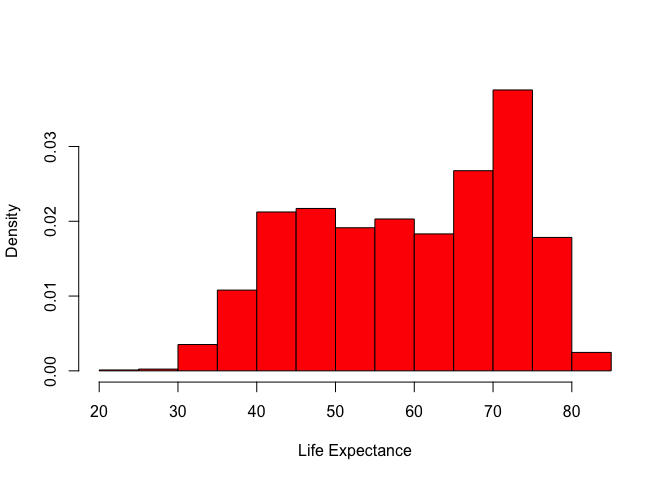
\includegraphics{GAPMIDER_files/figure-latex/unnamed-chunk-15-1.pdf}

\begin{Shaded}
\begin{Highlighting}[]
\NormalTok{##This graph shows the typical layout of a box-whisker plot.The stripe shows the median, the box represents the upper and lower hinges, and the whiskers show the maximum and minimum values.}
\end{Highlighting}
\end{Shaded}

\begin{Shaded}
\begin{Highlighting}[]
\KeywordTok{plot}\NormalTok{(gdpPercap }\OperatorTok{~}\StringTok{ }\NormalTok{lifeExp, }\DataTypeTok{xlab =} \StringTok{'Year'}\NormalTok{, }\DataTypeTok{ylab =} \StringTok{'life expetancy'}\NormalTok{,}\DataTypeTok{pch =} \DecValTok{18}\NormalTok{, }\DataTypeTok{cex =} \DecValTok{2}\NormalTok{, }\DataTypeTok{col =} \StringTok{'gray50'}\NormalTok{)}
 
\KeywordTok{abline}\NormalTok{(}\KeywordTok{lm}\NormalTok{(gdpPercap }\OperatorTok{~}\StringTok{ }\NormalTok{year), }\DataTypeTok{lty =} \StringTok{'dotted'}\NormalTok{, }\DataTypeTok{lwd =} \DecValTok{2}\NormalTok{, }\DataTypeTok{col =} \StringTok{'gray50'}\NormalTok{)}
\end{Highlighting}
\end{Shaded}

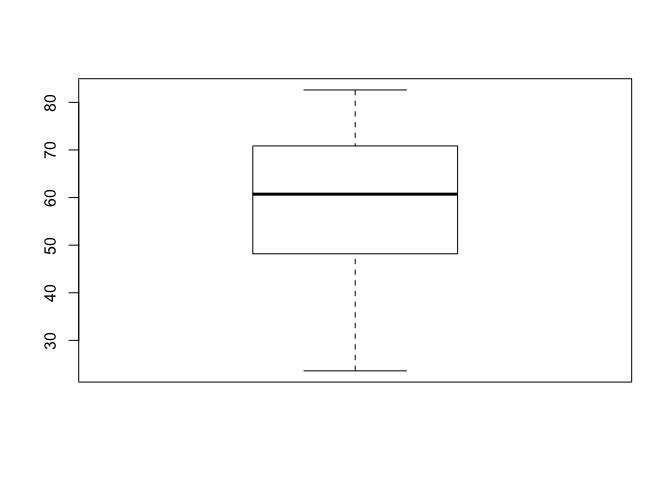
\includegraphics{GAPMIDER_files/figure-latex/unnamed-chunk-16-1.pdf}

\begin{Shaded}
\begin{Highlighting}[]
\KeywordTok{library}\NormalTok{(gapminder)}
\KeywordTok{library}\NormalTok{(tidyverse)}
\end{Highlighting}
\end{Shaded}

\begin{verbatim}
## -- Attaching packages ------------------------------------------------- tidyverse 1.2.1 --
\end{verbatim}

\begin{verbatim}
## √ ggplot2 3.0.0     √ purrr   0.2.5
## √ tibble  1.4.2     √ dplyr   0.7.6
## √ tidyr   0.8.1     √ stringr 1.3.1
## √ readr   1.1.1     √ forcats 0.3.0
\end{verbatim}

\begin{verbatim}
## Warning: package 'readr' was built under R version 3.3.2
\end{verbatim}

\begin{verbatim}
## -- Conflicts ---------------------------------------------------- tidyverse_conflicts() --
## x dplyr::filter() masks stats::filter()
## x dplyr::lag()    masks stats::lag()
\end{verbatim}

\begin{Shaded}
\begin{Highlighting}[]
\NormalTok{##Putting continent and country first and everything() after that.}

\KeywordTok{select}\NormalTok{(gapminder,continent,country,}\KeywordTok{everything}\NormalTok{())}
\end{Highlighting}
\end{Shaded}

\begin{verbatim}
## # A tibble: 1,704 x 6
##    continent country      year lifeExp      pop gdpPercap
##    <fct>     <fct>       <int>   <dbl>    <int>     <dbl>
##  1 Asia      Afghanistan  1952    28.8  8425333      779.
##  2 Asia      Afghanistan  1957    30.3  9240934      821.
##  3 Asia      Afghanistan  1962    32.0 10267083      853.
##  4 Asia      Afghanistan  1967    34.0 11537966      836.
##  5 Asia      Afghanistan  1972    36.1 13079460      740.
##  6 Asia      Afghanistan  1977    38.4 14880372      786.
##  7 Asia      Afghanistan  1982    39.9 12881816      978.
##  8 Asia      Afghanistan  1987    40.8 13867957      852.
##  9 Asia      Afghanistan  1992    41.7 16317921      649.
## 10 Asia      Afghanistan  1997    41.8 22227415      635.
## # ... with 1,694 more rows
\end{verbatim}

\begin{Shaded}
\begin{Highlighting}[]
\NormalTok{##Select columns country, pop,lifeExp from the gapminder data, in that order.}

\KeywordTok{select}\NormalTok{(gapminder,country,pop,lifeExp)}
\end{Highlighting}
\end{Shaded}

\begin{verbatim}
## # A tibble: 1,704 x 3
##    country          pop lifeExp
##    <fct>          <int>   <dbl>
##  1 Afghanistan  8425333    28.8
##  2 Afghanistan  9240934    30.3
##  3 Afghanistan 10267083    32.0
##  4 Afghanistan 11537966    34.0
##  5 Afghanistan 13079460    36.1
##  6 Afghanistan 14880372    38.4
##  7 Afghanistan 12881816    39.9
##  8 Afghanistan 13867957    40.8
##  9 Afghanistan 16317921    41.7
## 10 Afghanistan 22227415    41.8
## # ... with 1,694 more rows
\end{verbatim}

\begin{Shaded}
\begin{Highlighting}[]
\NormalTok{##Select all variables, from continent to pop}

\KeywordTok{select}\NormalTok{(gapminder,continent}\OperatorTok{:}\NormalTok{pop)}
\end{Highlighting}
\end{Shaded}

\begin{verbatim}
## # A tibble: 1,704 x 4
##    continent  year lifeExp      pop
##    <fct>     <int>   <dbl>    <int>
##  1 Asia       1952    28.8  8425333
##  2 Asia       1957    30.3  9240934
##  3 Asia       1962    32.0 10267083
##  4 Asia       1967    34.0 11537966
##  5 Asia       1972    36.1 13079460
##  6 Asia       1977    38.4 14880372
##  7 Asia       1982    39.9 12881816
##  8 Asia       1987    40.8 13867957
##  9 Asia       1992    41.7 16317921
## 10 Asia       1997    41.8 22227415
## # ... with 1,694 more rows
\end{verbatim}

\begin{Shaded}
\begin{Highlighting}[]
\NormalTok{##Select all columns except year}

\KeywordTok{select}\NormalTok{(gapminder,}\OperatorTok{-}\NormalTok{year)}
\end{Highlighting}
\end{Shaded}

\begin{verbatim}
## # A tibble: 1,704 x 5
##    country     continent lifeExp      pop gdpPercap
##    <fct>       <fct>       <dbl>    <int>     <dbl>
##  1 Afghanistan Asia         28.8  8425333      779.
##  2 Afghanistan Asia         30.3  9240934      821.
##  3 Afghanistan Asia         32.0 10267083      853.
##  4 Afghanistan Asia         34.0 11537966      836.
##  5 Afghanistan Asia         36.1 13079460      740.
##  6 Afghanistan Asia         38.4 14880372      786.
##  7 Afghanistan Asia         39.9 12881816      978.
##  8 Afghanistan Asia         40.8 13867957      852.
##  9 Afghanistan Asia         41.7 16317921      649.
## 10 Afghanistan Asia         41.8 22227415      635.
## # ... with 1,694 more rows
\end{verbatim}

\begin{Shaded}
\begin{Highlighting}[]
\NormalTok{##Select columns whose name starts with a character string. }

\KeywordTok{select}\NormalTok{(gapminder,}\KeywordTok{starts_with}\NormalTok{(}\StringTok{"life"}\NormalTok{))}
\end{Highlighting}
\end{Shaded}

\begin{verbatim}
## # A tibble: 1,704 x 1
##    lifeExp
##      <dbl>
##  1    28.8
##  2    30.3
##  3    32.0
##  4    34.0
##  5    36.1
##  6    38.4
##  7    39.9
##  8    40.8
##  9    41.7
## 10    41.8
## # ... with 1,694 more rows
\end{verbatim}

\begin{Shaded}
\begin{Highlighting}[]
\NormalTok{##Select columns whose name matches a regular expression. }

\KeywordTok{select}\NormalTok{(gapminder,}\KeywordTok{matches}\NormalTok{(}\StringTok{".l."}\NormalTok{))}
\end{Highlighting}
\end{Shaded}

\begin{verbatim}
## # A tibble: 1,704 x 0
\end{verbatim}

\begin{Shaded}
\begin{Highlighting}[]
\NormalTok{##Select columns whose name contains a character string. }

\KeywordTok{select}\NormalTok{(gapminder,}\KeywordTok{contains}\NormalTok{(}\StringTok{"."}\NormalTok{))}
\end{Highlighting}
\end{Shaded}

\begin{verbatim}
## # A tibble: 1,704 x 0
\end{verbatim}

\begin{Shaded}
\begin{Highlighting}[]
\NormalTok{##Select columns whose name starts with a character string. }

\KeywordTok{select}\NormalTok{(gapminder,}\KeywordTok{ends_with}\NormalTok{(}\StringTok{"p"}\NormalTok{))}
\end{Highlighting}
\end{Shaded}

\begin{verbatim}
## # A tibble: 1,704 x 3
##    lifeExp      pop gdpPercap
##      <dbl>    <int>     <dbl>
##  1    28.8  8425333      779.
##  2    30.3  9240934      821.
##  3    32.0 10267083      853.
##  4    34.0 11537966      836.
##  5    36.1 13079460      740.
##  6    38.4 14880372      786.
##  7    39.9 12881816      978.
##  8    40.8 13867957      852.
##  9    41.7 16317921      649.
## 10    41.8 22227415      635.
## # ... with 1,694 more rows
\end{verbatim}

\begin{Shaded}
\begin{Highlighting}[]
\NormalTok{##Select columns whose names are in a group of names. }

\KeywordTok{select}\NormalTok{(gapminder, }\KeywordTok{one_of}\NormalTok{(}\KeywordTok{c}\NormalTok{(}\StringTok{"country"}\NormalTok{, }\StringTok{"continent"}\NormalTok{)))}
\end{Highlighting}
\end{Shaded}

\begin{verbatim}
## # A tibble: 1,704 x 2
##    country     continent
##    <fct>       <fct>    
##  1 Afghanistan Asia     
##  2 Afghanistan Asia     
##  3 Afghanistan Asia     
##  4 Afghanistan Asia     
##  5 Afghanistan Asia     
##  6 Afghanistan Asia     
##  7 Afghanistan Asia     
##  8 Afghanistan Asia     
##  9 Afghanistan Asia     
## 10 Afghanistan Asia     
## # ... with 1,694 more rows
\end{verbatim}

\begin{Shaded}
\begin{Highlighting}[]
\NormalTok{## arrange() function}

\KeywordTok{arrange}\NormalTok{(gapminder,year)}
\end{Highlighting}
\end{Shaded}

\begin{verbatim}
## # A tibble: 1,704 x 6
##    country     continent  year lifeExp      pop gdpPercap
##    <fct>       <fct>     <int>   <dbl>    <int>     <dbl>
##  1 Afghanistan Asia       1952    28.8  8425333      779.
##  2 Albania     Europe     1952    55.2  1282697     1601.
##  3 Algeria     Africa     1952    43.1  9279525     2449.
##  4 Angola      Africa     1952    30.0  4232095     3521.
##  5 Argentina   Americas   1952    62.5 17876956     5911.
##  6 Australia   Oceania    1952    69.1  8691212    10040.
##  7 Austria     Europe     1952    66.8  6927772     6137.
##  8 Bahrain     Asia       1952    50.9   120447     9867.
##  9 Bangladesh  Asia       1952    37.5 46886859      684.
## 10 Belgium     Europe     1952    68    8730405     8343.
## # ... with 1,694 more rows
\end{verbatim}

\begin{Shaded}
\begin{Highlighting}[]
\KeywordTok{arrange}\NormalTok{(gapminder,}\KeywordTok{desc}\NormalTok{(lifeExp))}
\end{Highlighting}
\end{Shaded}

\begin{verbatim}
## # A tibble: 1,704 x 6
##    country          continent  year lifeExp       pop gdpPercap
##    <fct>            <fct>     <int>   <dbl>     <int>     <dbl>
##  1 Japan            Asia       2007    82.6 127467972    31656.
##  2 Hong Kong, China Asia       2007    82.2   6980412    39725.
##  3 Japan            Asia       2002    82   127065841    28605.
##  4 Iceland          Europe     2007    81.8    301931    36181.
##  5 Switzerland      Europe     2007    81.7   7554661    37506.
##  6 Hong Kong, China Asia       2002    81.5   6762476    30209.
##  7 Australia        Oceania    2007    81.2  20434176    34435.
##  8 Spain            Europe     2007    80.9  40448191    28821.
##  9 Sweden           Europe     2007    80.9   9031088    33860.
## 10 Israel           Asia       2007    80.7   6426679    25523.
## # ... with 1,694 more rows
\end{verbatim}

\begin{Shaded}
\begin{Highlighting}[]
\KeywordTok{arrange}\NormalTok{(gapminder,pop,lifeExp)}
\end{Highlighting}
\end{Shaded}

\begin{verbatim}
## # A tibble: 1,704 x 6
##    country               continent  year lifeExp   pop gdpPercap
##    <fct>                 <fct>     <int>   <dbl> <int>     <dbl>
##  1 Sao Tome and Principe Africa     1952    46.5 60011      880.
##  2 Sao Tome and Principe Africa     1957    48.9 61325      861.
##  3 Djibouti              Africa     1952    34.8 63149     2670.
##  4 Sao Tome and Principe Africa     1962    51.9 65345     1072.
##  5 Sao Tome and Principe Africa     1967    54.4 70787     1385.
##  6 Djibouti              Africa     1957    37.3 71851     2865.
##  7 Sao Tome and Principe Africa     1972    56.5 76595     1533.
##  8 Sao Tome and Principe Africa     1977    58.6 86796     1738.
##  9 Djibouti              Africa     1962    39.7 89898     3021.
## 10 Sao Tome and Principe Africa     1982    60.4 98593     1890.
## # ... with 1,694 more rows
\end{verbatim}

\begin{Shaded}
\begin{Highlighting}[]
\NormalTok{## Piping, `%>%`}

\NormalTok{gapminder }\OperatorTok\StringTok{ }
\StringTok{  }\KeywordTok{select}\NormalTok{(year,lifeExp,country) }\OperatorTok\StringTok{ }
\StringTok{  }\KeywordTok{arrange}\NormalTok{(year,lifeExp)}
\end{Highlighting}
\end{Shaded}

\begin{verbatim}
## # A tibble: 1,704 x 3
##     year lifeExp country      
##    <int>   <dbl> <fct>        
##  1  1952    28.8 Afghanistan  
##  2  1952    30   Gambia       
##  3  1952    30.0 Angola       
##  4  1952    30.3 Sierra Leone 
##  5  1952    31.3 Mozambique   
##  6  1952    32.0 Burkina Faso 
##  7  1952    32.5 Guinea-Bissau
##  8  1952    32.5 Yemen, Rep.  
##  9  1952    33.0 Somalia      
## 10  1952    33.6 Guinea       
## # ... with 1,694 more rows
\end{verbatim}

\begin{Shaded}
\begin{Highlighting}[]
\NormalTok{## filter()}

\KeywordTok{filter}\NormalTok{(gapminder, pop }\OperatorTok{>}\StringTok{ }\DecValTok{7}\NormalTok{)}
\end{Highlighting}
\end{Shaded}

\begin{verbatim}
## # A tibble: 1,704 x 6
##    country     continent  year lifeExp      pop gdpPercap
##    <fct>       <fct>     <int>   <dbl>    <int>     <dbl>
##  1 Afghanistan Asia       1952    28.8  8425333      779.
##  2 Afghanistan Asia       1957    30.3  9240934      821.
##  3 Afghanistan Asia       1962    32.0 10267083      853.
##  4 Afghanistan Asia       1967    34.0 11537966      836.
##  5 Afghanistan Asia       1972    36.1 13079460      740.
##  6 Afghanistan Asia       1977    38.4 14880372      786.
##  7 Afghanistan Asia       1982    39.9 12881816      978.
##  8 Afghanistan Asia       1987    40.8 13867957      852.
##  9 Afghanistan Asia       1992    41.7 16317921      649.
## 10 Afghanistan Asia       1997    41.8 22227415      635.
## # ... with 1,694 more rows
\end{verbatim}

\begin{Shaded}
\begin{Highlighting}[]
\NormalTok{##Extract rows that meet logical criteria. }
\end{Highlighting}
\end{Shaded}

\begin{Shaded}
\begin{Highlighting}[]
\KeywordTok{mean}\NormalTok{(lifeExp) }
\end{Highlighting}
\end{Shaded}

\begin{verbatim}
## [1] 59.47444
\end{verbatim}

\begin{Shaded}
\begin{Highlighting}[]
\NormalTok{gapminder }\OperatorTok\StringTok{ }
\KeywordTok{filter}\NormalTok{(lifeExp}\OperatorTok{>}\KeywordTok{mean}\NormalTok{(lifeExp) )  }
\end{Highlighting}
\end{Shaded}

\begin{verbatim}
## # A tibble: 895 x 6
##    country continent  year lifeExp     pop gdpPercap
##    <fct>   <fct>     <int>   <dbl>   <int>     <dbl>
##  1 Albania Europe     1962    64.8 1728137     2313.
##  2 Albania Europe     1967    66.2 1984060     2760.
##  3 Albania Europe     1972    67.7 2263554     3313.
##  4 Albania Europe     1977    68.9 2509048     3533.
##  5 Albania Europe     1982    70.4 2780097     3631.
##  6 Albania Europe     1987    72   3075321     3739.
##  7 Albania Europe     1992    71.6 3326498     2497.
##  8 Albania Europe     1997    73.0 3428038     3193.
##  9 Albania Europe     2002    75.7 3508512     4604.
## 10 Albania Europe     2007    76.4 3600523     5937.
## # ... with 885 more rows
\end{verbatim}

\begin{Shaded}
\begin{Highlighting}[]
\NormalTok{gapminder }\OperatorTok\StringTok{ }
\StringTok{  }\KeywordTok{select}\NormalTok{(country,continent) }\OperatorTok\StringTok{ }
\StringTok{  }\KeywordTok{filter}\NormalTok{(year}\OperatorTok{>=}\DecValTok{1960} \OperatorTok{&}\StringTok{ }\NormalTok{year}\OperatorTok{<}\DecValTok{1970}\NormalTok{ )}
\end{Highlighting}
\end{Shaded}

\begin{verbatim}
## # A tibble: 284 x 2
##    country     continent
##    <fct>       <fct>    
##  1 Afghanistan Asia     
##  2 Afghanistan Asia     
##  3 Albania     Europe   
##  4 Albania     Europe   
##  5 Algeria     Africa   
##  6 Algeria     Africa   
##  7 Angola      Africa   
##  8 Angola      Africa   
##  9 Argentina   Americas 
## 10 Argentina   Americas 
## # ... with 274 more rows
\end{verbatim}

\begin{Shaded}
\begin{Highlighting}[]
\NormalTok{gapminder }\OperatorTok\StringTok{ }
\StringTok{  }\KeywordTok{filter}\NormalTok{((country}\OperatorTok{==}\StringTok{"Afganistan"}\OperatorTok{|}\StringTok{ }\NormalTok{country}\OperatorTok{==}\StringTok{"Canada"}\NormalTok{) }\OperatorTok{&}\StringTok{ }\NormalTok{gdpPercap}\OperatorTok{>=}\DecValTok{10000} \OperatorTok{&}\StringTok{ }\NormalTok{year}\OperatorTok{<}\DecValTok{22000}\NormalTok{ )}
\end{Highlighting}
\end{Shaded}

\begin{verbatim}
## # A tibble: 12 x 6
##    country continent  year lifeExp      pop gdpPercap
##    <fct>   <fct>     <int>   <dbl>    <int>     <dbl>
##  1 Canada  Americas   1952    68.8 14785584    11367.
##  2 Canada  Americas   1957    70.0 17010154    12490.
##  3 Canada  Americas   1962    71.3 18985849    13462.
##  4 Canada  Americas   1967    72.1 20819767    16077.
##  5 Canada  Americas   1972    72.9 22284500    18971.
##  6 Canada  Americas   1977    74.2 23796400    22091.
##  7 Canada  Americas   1982    75.8 25201900    22899.
##  8 Canada  Americas   1987    76.9 26549700    26627.
##  9 Canada  Americas   1992    78.0 28523502    26343.
## 10 Canada  Americas   1997    78.6 30305843    28955.
## 11 Canada  Americas   2002    79.8 31902268    33329.
## 12 Canada  Americas   2007    80.7 33390141    36319.
\end{verbatim}

\begin{Shaded}
\begin{Highlighting}[]
\NormalTok{gapminder }\OperatorTok\StringTok{ }
\StringTok{  }\KeywordTok{filter}\NormalTok{(country }\OperatorTok\StringTok{ }\KeywordTok{c}\NormalTok{(}\StringTok{"India"}\NormalTok{,}\StringTok{"Angola"}\NormalTok{), year}\OperatorTok{>=}\DecValTok{1950}\NormalTok{, year}\OperatorTok{<}\DecValTok{1980}\NormalTok{)}
\end{Highlighting}
\end{Shaded}

\begin{verbatim}
## # A tibble: 12 x 6
##    country continent  year lifeExp       pop gdpPercap
##    <fct>   <fct>     <int>   <dbl>     <int>     <dbl>
##  1 Angola  Africa     1952    30.0   4232095     3521.
##  2 Angola  Africa     1957    32.0   4561361     3828.
##  3 Angola  Africa     1962    34     4826015     4269.
##  4 Angola  Africa     1967    36.0   5247469     5523.
##  5 Angola  Africa     1972    37.9   5894858     5473.
##  6 Angola  Africa     1977    39.5   6162675     3009.
##  7 India   Asia       1952    37.4 372000000      547.
##  8 India   Asia       1957    40.2 409000000      590.
##  9 India   Asia       1962    43.6 454000000      658.
## 10 India   Asia       1967    47.2 506000000      701.
## 11 India   Asia       1972    50.7 567000000      724.
## 12 India   Asia       1977    54.2 634000000      813.
\end{verbatim}

\hypertarget{scatterplot}{%
\subsection{Scatterplot}\label{scatterplot}}

A \emph{scatterplot} of \texttt{gdpPercap} vs. \texttt{year}.

\begin{longtable}[]{@{}ll@{}}
\toprule
Grammar Component & Specification\tabularnewline
\midrule
\endhead
\textbf{data} & \texttt{gapminder}\tabularnewline
\textbf{aesthetic mapping} & \texttt{x} and \texttt{y}\tabularnewline
\textbf{geometric object} & point\tabularnewline
scale & linear\tabularnewline
statistical transform & none\tabularnewline
coordinate system & rectangular\tabularnewline
facetting & none\tabularnewline
\bottomrule
\end{longtable}

\begin{Shaded}
\begin{Highlighting}[]
\KeywordTok{ggplot}\NormalTok{(gapminder,}\KeywordTok{aes}\NormalTok{(}\DataTypeTok{x=}\NormalTok{year,}\DataTypeTok{y=}\NormalTok{gdpPercap))}\OperatorTok{+}
\StringTok{  }\KeywordTok{geom_point}\NormalTok{(}\DataTypeTok{color=}\StringTok{"orange"}\NormalTok{)}
\end{Highlighting}
\end{Shaded}

\includegraphics{GAPMIDER_files/figure-latex/unnamed-chunk-34-1.pdf}

\begin{Shaded}
\begin{Highlighting}[]
\NormalTok{a<-}\StringTok{ }\KeywordTok{ggplot}\NormalTok{(gapminder,}\KeywordTok{aes}\NormalTok{(lifeExp))}\OperatorTok{+}
\StringTok{  }\KeywordTok{scale_y_log10}\NormalTok{()}
\NormalTok{a}\OperatorTok{+}\KeywordTok{geom_histogram}\NormalTok{(}\DataTypeTok{bins=}\DecValTok{50}\NormalTok{,}\DataTypeTok{color=}\StringTok{"red"}\NormalTok{)}
\end{Highlighting}
\end{Shaded}

\begin{verbatim}
## Warning: Transformation introduced infinite values in continuous y-axis
\end{verbatim}

\begin{verbatim}
## Warning: Removed 3 rows containing missing values (geom_bar).
\end{verbatim}

\includegraphics{GAPMIDER_files/figure-latex/unnamed-chunk-35-1.pdf}

\begin{Shaded}
\begin{Highlighting}[]
\NormalTok{b<-}\StringTok{ }\KeywordTok{ggplot}\NormalTok{(gapminder,}\KeywordTok{aes}\NormalTok{(continent,lifeExp))}\OperatorTok{+}
\StringTok{  }\KeywordTok{scale_y_log10}\NormalTok{()}
\NormalTok{b}
\end{Highlighting}
\end{Shaded}

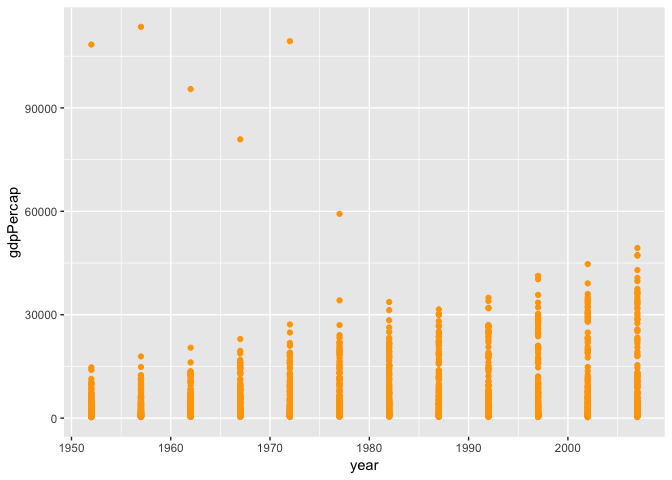
\includegraphics{GAPMIDER_files/figure-latex/unnamed-chunk-36-1.pdf}

\begin{Shaded}
\begin{Highlighting}[]
\NormalTok{b}\OperatorTok{+}\KeywordTok{geom_violin}\NormalTok{()}
\end{Highlighting}
\end{Shaded}

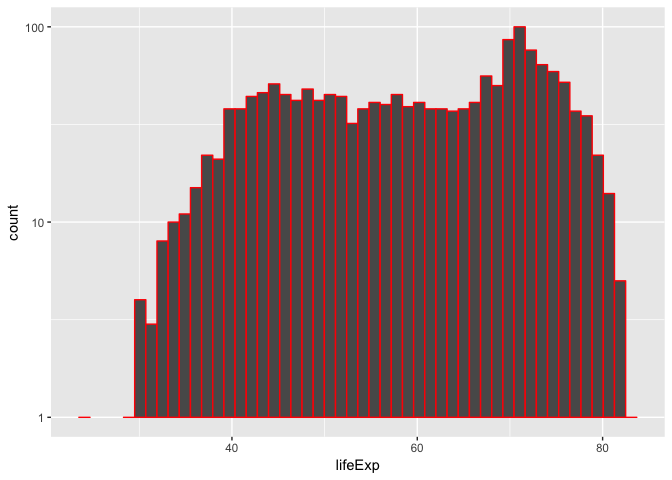
\includegraphics{GAPMIDER_files/figure-latex/unnamed-chunk-37-1.pdf}

\begin{Shaded}
\begin{Highlighting}[]
\NormalTok{b}\OperatorTok{+}\KeywordTok{geom_violin}\NormalTok{()}\OperatorTok{+}
\StringTok{  }\KeywordTok{geom_jitter}\NormalTok{(}\DataTypeTok{alpha=}\FloatTok{0.5}\NormalTok{)}
\end{Highlighting}
\end{Shaded}

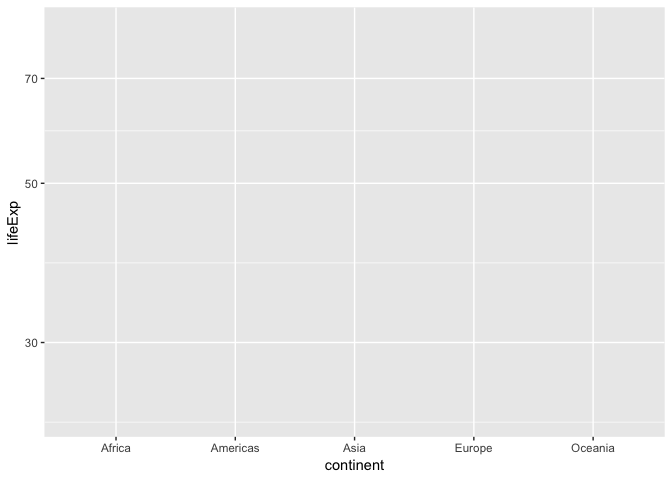
\includegraphics{GAPMIDER_files/figure-latex/unnamed-chunk-38-1.pdf}

\begin{Shaded}
\begin{Highlighting}[]
\NormalTok{gapminder }\OperatorTok\StringTok{ }
\StringTok{  }\KeywordTok{filter}\NormalTok{(country}\OperatorTok{==}\StringTok{"India"}\NormalTok{) }\OperatorTok\StringTok{ }
\StringTok{  }\KeywordTok{ggplot}\NormalTok{(}\KeywordTok{aes}\NormalTok{(year,gdpPercap)) }\OperatorTok{+}
\StringTok{  }\KeywordTok{geom_line}\NormalTok{()}\OperatorTok{+}
\StringTok{  }\KeywordTok{geom_point}\NormalTok{(}\DataTypeTok{color=}\StringTok{"blue"}\NormalTok{)}
\end{Highlighting}
\end{Shaded}

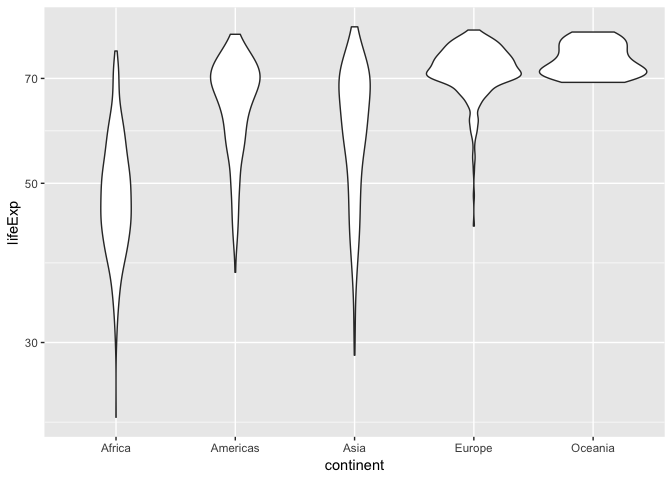
\includegraphics{GAPMIDER_files/figure-latex/unnamed-chunk-39-1.pdf}


\end{document}
